\documentclass[preprint, 3p,
authoryear]{elsarticle} %review=doublespace preprint=single 5p=2 column
%%% Begin My package additions %%%%%%%%%%%%%%%%%%%

\usepackage[hyphens]{url}

  \journal{Transport Geography?} % Sets Journal name

\usepackage{graphicx}
%%%%%%%%%%%%%%%% end my additions to header

\usepackage[T1]{fontenc}
\usepackage{lmodern}
\usepackage{amssymb,amsmath}
% TODO: Currently lineno needs to be loaded after amsmath because of conflict
% https://github.com/latex-lineno/lineno/issues/5
\usepackage{lineno} % add
\usepackage{ifxetex,ifluatex}
\usepackage{fixltx2e} % provides \textsubscript
% use upquote if available, for straight quotes in verbatim environments
\IfFileExists{upquote.sty}{\usepackage{upquote}}{}
\ifnum 0\ifxetex 1\fi\ifluatex 1\fi=0 % if pdftex
  \usepackage[utf8]{inputenc}
\else % if luatex or xelatex
  \usepackage{fontspec}
  \ifxetex
    \usepackage{xltxtra,xunicode}
  \fi
  \defaultfontfeatures{Mapping=tex-text,Scale=MatchLowercase}
  \newcommand{\euro}{€}
\fi
% use microtype if available
\IfFileExists{microtype.sty}{\usepackage{microtype}}{}
\usepackage[]{natbib}
\bibliographystyle{plainnat}

\usepackage{graphicx}
\ifxetex
  \usepackage[setpagesize=false, % page size defined by xetex
              unicode=false, % unicode breaks when used with xetex
              xetex]{hyperref}
\else
  \usepackage[unicode=true]{hyperref}
\fi
\hypersetup{breaklinks=true,
            bookmarks=true,
            pdfauthor={},
            pdftitle={Leveraging GTFS to explore spatial patterns in transit supply with respect to social needs},
            colorlinks=false,
            urlcolor=blue,
            linkcolor=magenta,
            pdfborder={0 0 0}}

\setcounter{secnumdepth}{5}
% Pandoc toggle for numbering sections (defaults to be off)


% tightlist command for lists without linebreak
\providecommand{\tightlist}{%
  \setlength{\itemsep}{0pt}\setlength{\parskip}{0pt}}




\usepackage{subfig}
\usepackage{booktabs}
\usepackage{longtable}
\usepackage{array}
\usepackage{multirow}
\usepackage{wrapfig}
\usepackage{float}
\usepackage{colortbl}
\usepackage{pdflscape}
\usepackage{tabu}
\usepackage{threeparttable}
\usepackage{threeparttablex}
\usepackage[normalem]{ulem}
\usepackage{makecell}
\usepackage{xcolor}



\begin{document}


\begin{frontmatter}

  \title{Leveraging GTFS to explore spatial patterns in transit supply
with respect to social needs}
    \author[Public Transport Research Group (PTRG)]{James Reynolds%
  %
  \fnref{1}}
   \ead{james.reynolds@monash.edu} 
    \author[Public Transport Research Group (PTRG)]{Graham Currie%
  \corref{cor1}%
  \fnref{2}}
   \ead{graham.currie@monash.edu} 
    \author[Public Transport Research Group (PTRG)]{Yanda Qu%
  %
  \fnref{3}}
   \ead{yanda.qu@monash.edu} 
      \affiliation[Public Transport Research Group (PTRG)]{
    organization={Public Transport Research Group (PTRG), Institute of
Transport Studies, Department of Civil Engineering Engineering, Monash
University},addressline={Clayton
Campus},city={Melbourne},postcode={3800},state={Victoria},country={Australia},}
    \cortext[cor1]{Corresponding author}
    \fntext[1]{Research Fellow}
    \fntext[2]{Professor}
    \fntext[3]{PhD Student}
  
  \begin{abstract}
  This is the abstract.

  It consists of two paragraphs.
  \end{abstract}
    \begin{keyword}
    keyword1 \sep 
    keyword2
  \end{keyword}
  
 \end{frontmatter}

\section{Introduction}\label{introduction}

Providing basic mobility for those who cannot otherwise drive is a key
purpose for transit in many places \citep{Currie:2016aa}. Age,
disability, socio-economic status, lack of a driver's license or
vehicle, and many other factors might make someone reliant on transit
services for some or all of their travel. An approach for identifying
spatial gaps in transit supply, where is a high or very high social need
yet little or no service, was reported in \citet{Currie2003Hobart},
\citet{Currie2004Gap}, \citet{Currie2007Identifying} and
\citet{currie2010identifying}. However, there does not appear to have
been much further use or development of this approach. As well, it is
unclear if the spatial patterns identified in this previous research are
representative of transit supply and social need in other places, or
whether the location of gaps have changed in the intervening years.

This may in part be because until recently schedule data was not readily
available in consistent, electronic formats, meaning that assessing
transit supply was a large task. Nowadays, more than 10,000 transit
agencies publicly release data in the General Transit Feed Specification
(GTFS) format \citep{GTFS}. However, software tools for examining
spatial patterns and gaps in transit supply with respect to social needs
for transport do not appear to be readily available. This gap, and the
lack of direct follow up to \citet{Currie2003Hobart},
\citet{Currie2004Gap}, \citet{Currie2007Identifying} and
\citet{currie2010identifying}, provide the motivation for this paper.

The three main objectives of this research are: (1) to develop tools for
undertaking needs-gap analysis using GTFS datasets; (2) to explore
whether such gaps in Melbourne have changed since the publication of
\citet{Currie2007Identifying} and \citet{currie2010identifying}; and (3)
to better understand whether spatial patterns in Melbourne are
representative of those in other places. Outcomes of this research
reported in this paper include the development of a new R package
(gtfssupplyindex) with software tools that facilitate the use of the
\citet{Currie2003Hobart}, \citet{Currie2004Gap},
\citet{Currie2007Identifying} and \citet{currie2010identifying}
approach, in particular the calculation of transit Supply Index (SI)
scores from GTFS datasets. Also presented in this paper are results for
Australian cities in 2016 and 2021, matching the most recent censuses,
which are compared across locations and to the 2006 analysis of
Melbourne reported in \citet{currie2010identifying}.

The remainder of this paper is structured as follows: the next section
outlines the background to this research. Section 3 describes the study
methodology, followed by presentation of results in Section 4 and
discussion in Section 5. Limitations of this study, directions for
future research and a brief conclusion are provided in Section 6.

\section{Background}\label{background}

\subsection{Transit metrics}\label{transit-metrics}

There are many metrics available for benchmarking transit services.
These include those in the Transit Cooperative Research Program (TCRP)
Report 88, a guidebook for developing performance-measurement systems
\citep{Ryus:2003aa}; and those used across benchmarking databases and
programs such as \citet{Florida-Transit-Information-System:2018aa},
\citet{UITP:2015aa} and \citet{Imperial-College-London:2023aa}. The
Fielding Triangle \citep{FieldingGordonJ1987Mpts} provides a framework
for combining indicators of service inputs, outputs and consumption to
describe cost efficiency, cost effectiveness and service effectiveness.
More broadly: \citet{Litman:2003ab} and \citet{Litman:2016aa} discuss
some of the traffic, mobility, accessibility, social equity, strategic
planning and other rational decision-making-based perspectives
underlying many transport indicators; \citet{Reynolds:2017ah} extends
these into models of how institutionalism, incrementalism and other
public policy analysis concepts might apply to decision-making processes
relating to transit prioritization; \citet{GuzmanLuisA.2017Aeit}
developed a measure of accessibility in the context of policy
development and social equity for Latin American Bus Rapid Transit (BRT)
networks; and \citet{Creutzig2020streetspaceallocation} introduced
street space allocation metrics based around ten ethical principles.

However, many of these metrics may be difficult to calculate, explain or
understand, especially for those who are not planners, engineers or
other technical specialists. Where pre-calculated transit metrics are
immediately available, such as on a website or other online platform, it
may not be possible to independently generate scores, for instance to
assess proposed system changes. Contrasting examples are provided by:

\begin{itemize}
\item
  Transit Scores\citep{WalkScore:2023tg}, which are readily available
  online for locations with a published GTFS feed. The meaning of the
  metric also appears easy to explain, with the highest possible score
  of 100 representing the sort of transit accessibility experienced in
  the center of New York. However, the Transit Score algorithm is
  secret, and scores cannot be calculated independently or generated for
  proposed changes to networks.
\item
  The Transit Capacity and Quality of Service Manual (TCQSM), whic
  provides a wide range of metrics for measuring different aspects of a
  transit system. The TCQSM scores themselves appear easy to understand
  or explain, ranging from A (good) to F (bad), although the large
  number of metrics might be somewhat overwhelming for some users. The
  scores, however, can be calculated independently, given sufficient
  data.
\end{itemize}

The widespread availability of GTFS datasets in recent years has
facilitated the development of tools, such as the Transit Score, that
apply the same metric to many transit systems. \citet{Wong:2013aa}
provides another example of what can be done with GTFS data, open
metrics and coding, by reporting the distribution of various TCQSM
metrics across 50 USA transit operators. Code used in the
\citet{Wong:2013aa} analysis is available for those who might wish to
produce a similar study for other locations and systems. Developing a
similar code base, but for calculating metrics associated with spatial
gaps in transit supply based on social needs, is the subject of this
paper.

\subsection{The Transit Suppy Index}\label{the-transit-suppy-index}

An objective of this study is to produce code that facilitates
calculation of the SI metric from GTFS data. A generalized form of the
SI equation, adapted from \citet{currie2010identifying}, is:

\[SI_{area, time} = \sum{\frac{Area_{Bn}}{Area_{area}}*SL_{n, time}}\]

where:

\begin{itemize}
\item
  \(SI_{area, time}\) is the Supply Index for the area of interest and a
  given period of time;
\item
  \(Area_{Bn}\) is the buffer area for each stop (n) within the area of
  interest (in \citet{currie2010identifying} this was based on a radius
  of 400 metres for bus and tram stops, and 800 metres for railway
  stations);
\item
  \(Area_{area}\) is the area of the area of interest; and
\item
  \(SL_{n,time}\) is the number of transit arrivals for each stop for a
  given time period.
\end{itemize}

\begin{figure}
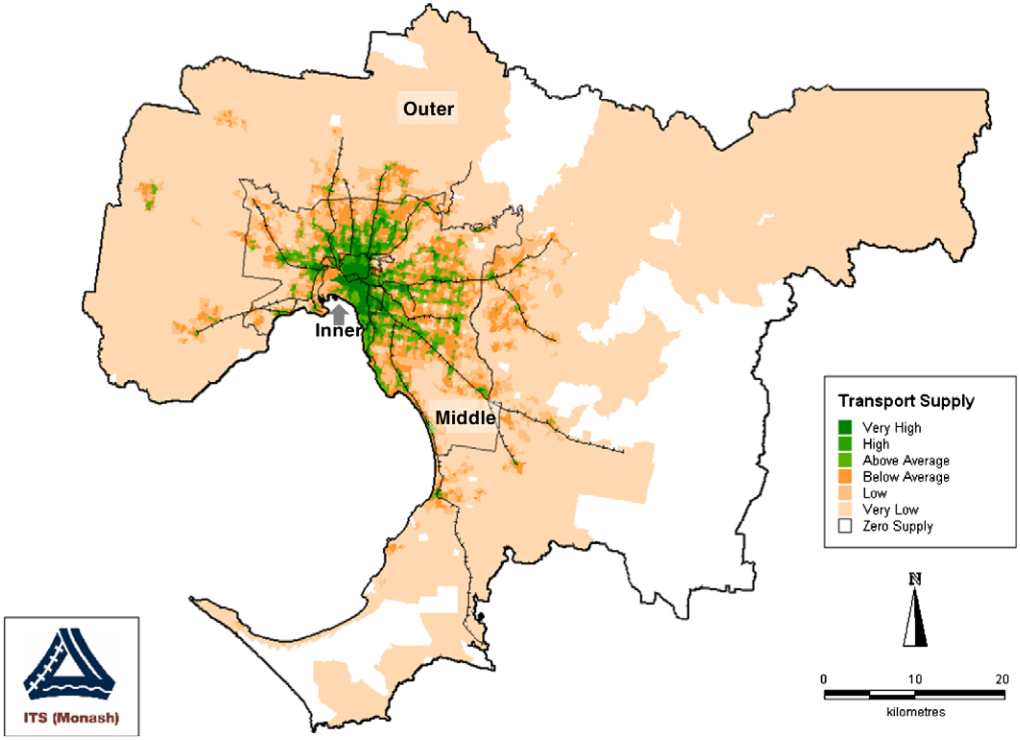
\includegraphics[width=1\linewidth]{graphics/Currie2010SI} \caption{Distribution of supply measure scores – Metropolitan Melbourne (2006), Source: Currie (2010)}\label{fig:Currie_map_SI}
\end{figure}

\citet{currie2010identifying} reported SI scores for Census Collection
Districts (CCDs) across Greater Melbourne in 2006, as shown in Figure
\ref{fig:Currie_map_SI}. General patterns were identified, being: more
transit supply in the middle and inner suburbs, and along passenger
railway lines; and outer areas tending to have very low SI scores or no
transit supply at all.

\subsection{Social need and needs gap}\label{social-need-and-needs-gap}

\begin{figure}
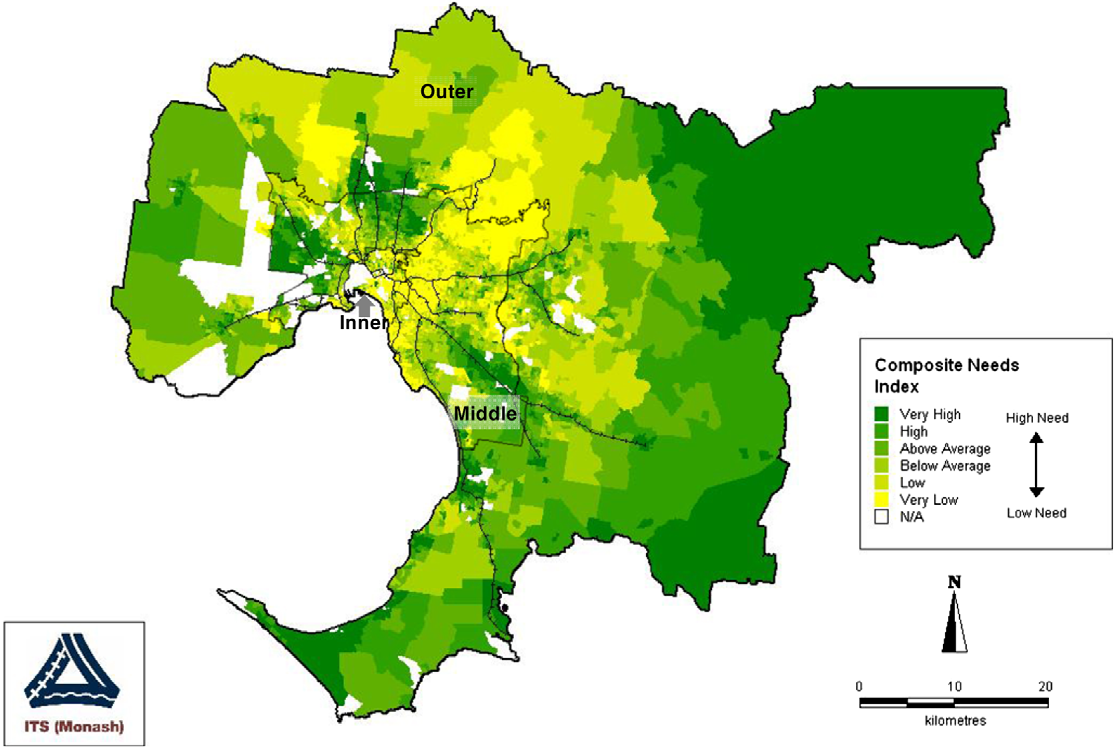
\includegraphics[width=1\linewidth]{graphics/Currie2010Needs} \caption{Distribution of categories of composite social need index scores in 2006. Source: Currie (2010.)}\label{fig:Currie_map_needs}
\end{figure}

As well as measuring transit supply, \citet{currie2010identifying}
assessed the social need for transit across Greater Melbourne using: the
Australian Bureaus of Statistics' Index of Related Socio-Economic
Advantage/Disadvantage (IRSAD) and a transport needs index derived from
eight weighted indicators. The spatial distribution of this composite
social needs index in 2006, reproduced in Figure
\textbackslash ref\{fig:Currie\_map\_needs), showed that areas of above
average, high and very high social needs in 2006 were located in: some
outer areas, particularly in the east and south-east; and in some middle
areas in the south-east, north and west.

As the final step in the spatial needs-gap analysis,
\citet{currie2010identifying} identified areas with very high transport
needs, but very low or no transit supply, as reproduced in Figure
\ref{fig:Currie_map_gap}. These areas were identified as being those
where service gaps might be of particular concern. Most of these were
located in outer parts of Melbourne in the north-east, south-east and
south, although there were also some pockets in the middle suburbs in
the west, north and south east. Overall, \citet{currie2010identifying}
found that ``8.2\% of Melbourne residents have `very high' needs but
`zero', `low' or `very low' public transport supply.''

\begin{figure}
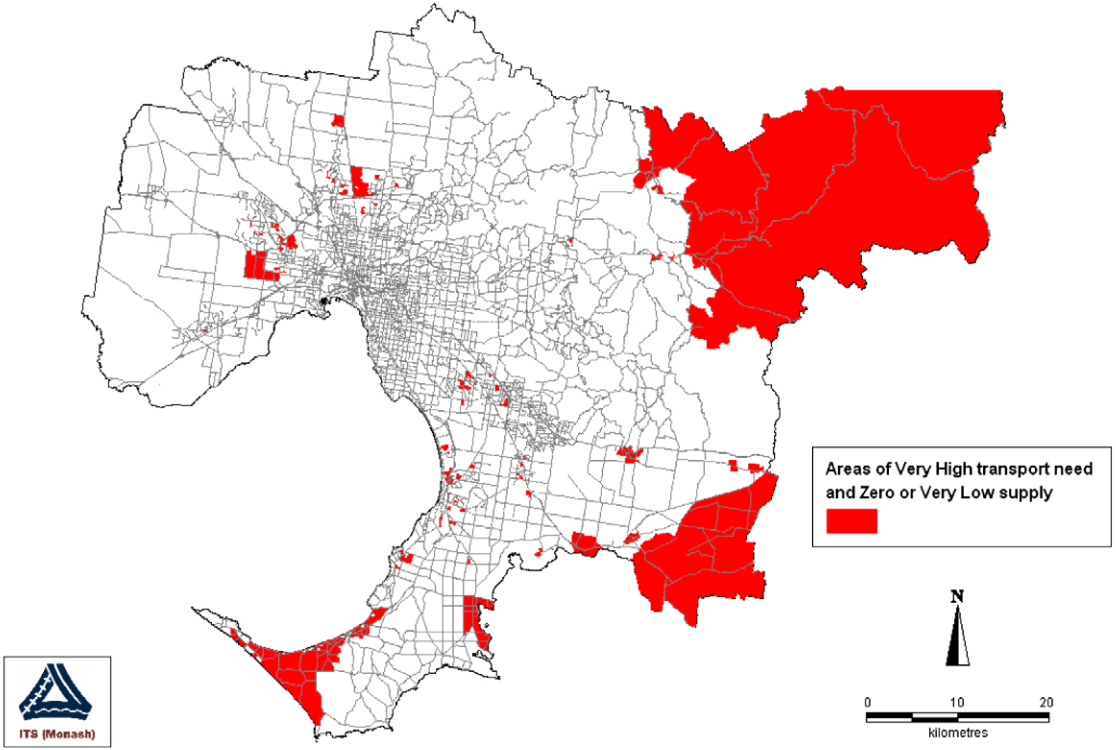
\includegraphics[width=1\linewidth]{graphics/Currie2010gap} \caption{Melbourne needs-gap in 2006 – very high transport need areas with zero or very low public transport supply, Source: Currie (2010)}\label{fig:Currie_map_gap}
\end{figure}

Using this methodology in transit planning was suggested as
``substantially more useful than the presentation of anecdotal evidence,
which is the most common means of identifying transport needs in local
transport studies throughout the world''\citep{currie2010identifying}.
However, it does not appear that this approach has been widely adopted
in practice or by researchers. Our suspicion is that while the SI has a
relatively simple formula and requires only geographic and timetable
data to calculate, the lack of software tools may be partly why it has
not been more widely adopted.

It is also unclear whether the patterns in Melbourne identified in
\citet{currie2010identifying} have changed since the 2006 analysis, or
if Melbourne is representative of other locations. Developing a software
tool to calculate SI tools from GTFS data, and then using it to
comparing current conditions and other locations to the findings of
\citet{currie2010identifying}, therefore, provides the motivation for
this research.

\section{Methodology}\label{methodology}

\subsection{Code development}\label{code-development}

This study developed a package of tools for calculating the SI from GTFS
data using the R programming language \citep{R-base}. The
recommendations of \citet{wickham2023r} informed the package setup and
development approach. Various existing packages and code examples were
relied upon including: the sf package \citep{R-sf} for geospatial
analysis; the tidyverse \citep{tidyverse2019}; gtfstools
\citep{R-gtfstools}; and tidytransit \citep{R-tidytransit}. Australian
Bureau of Statistics (ABS) data was also used, sourced via the strayr
and absmapsdata packages \citep{r-strayr}.

Code was developed and tested on the Mornington Peninsula Tourist
Railway GTFS feed. This was selected primarily for convenience, given
that the authors are familiar with the surrounding geography and that
the feed covers a small number of trips across just three stations.

\subsection{Changes since 2006: Greater
Melbourne}\label{changes-since-2006-greater-melbourne}

Much has changed since 2006, including the spatial geography used by the
Australian Bureau of Statistics (ABS) to collect census data. To allow
direct comparison between 2006 and the most recent census, therefore,
this study calculated SI scores using the same Census Collection
Districts (CCDs) used by \citet{currie2010identifying} for the week
starting the day of the 2021 census. The Victorian GTFS feed, published
by Public Transport Victoria (PTV), was used with historical feeds
sourced via \citet{transitfeeds_victoria:2023aa}.

Unfortunately, it is not possible to obtain 2016 or 2021 social
disadvantage data for CCDs, as the ABS no longer uses this geographic
scheme. Population and other statistics are now released for Statistical
Area 1 (SA1) zones, and so SI scores and needs-gap analysis was
completed for Greater Melbourne in 2021 using these boundaries instead.

\subsection{Variation in spatial patterns across
location.}\label{variation-in-spatial-patterns-across-location.}

SI scores were also calculated for other capital cities in Australia,
again for the week starting on the day of the 2021 census. Historical
GTFS data was again sourced via the Transit Feeds website. Unfortunately
it was not possible to locate historical GTFS data for Greater Sydney or
Greater Darwin, so SI scores were calculated for 2024 using the latest
data sets, sourced directly from the relevant transit authorities.

\subsection{Variation in time}\label{variation-in-time}

SHOULD THIS BE RUN FOR ALL YEARS AS FAR BACK AS THE GTFS DATA GOES??

\subsection{Measuring social
disadvantage}\label{measuring-social-disadvantage}

This study adopts a similar approach to measuring social disadvantage as
used in \citet{currie2010identifying}, using: the ABS' Index of Relative
Socio-Economic Advantage/Disadvantage (IRSAD); and a transport needs
index\footnote{The same need indicators and weightings used in
  \citet{currie2010identifying} were adopted, although \$799 or lower
  per week was used as the threshold for low income households rather
  than \$499 to account for inflation (as per Reserve Bank of
  Australia's online inflation calculator).}. A composite needs
indicator was derived based on the IRSAD and the transport needs index,
again as per the \citet{currie2010identifying} approach\footnote{However,
  changes to the ABS reporting systems mean that the composite needs
  indicator had to based on weighting both the IRSAD index and the
  transport need index by the total population of each SA1 zone, which
  were then added, standardised and split into six groups.}.

\section{Results}\label{results}

\subsection{The gtfssupplyindex
Package}\label{the-gtfssupplyindex-package}

Code developed to calculate SI scores is available as an R package on
github (see \citet{gtfssupplyindex_github}). Included in the package is
a vignette that outlines the structure of the calculations, the
developed functions (LINK HERE), and step-by-step calculations for the
Mornington Peninsula Railway as a worked example and comparison to SI
scores calculated manually.

\subsection{Greater Melbourne: changes since
2006}\label{greater-melbourne-changes-since-2006}

Figure \ref{fig:Greater_Melbourne_SA1_2021_plot} shows Transit Supply
groupings based on SI scores for SA1 zones within Greater Melbourne for
the week starting the day of the 2021 census. The 2006 boundary of
Greater Melbourne and the inner, middle and outer suburban boundaries
used by \citet{currie2010identifying} are also shown so as to facilitate
comparison to Figure \ref{fig:Currie_map_SI}.

\begin{figure}
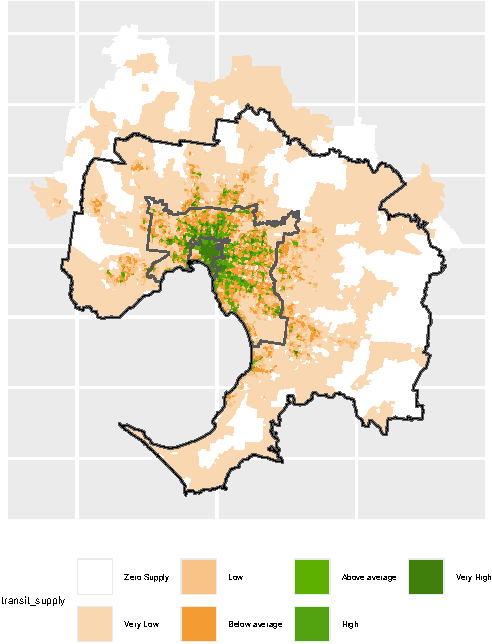
\includegraphics[width=1\linewidth]{Leveraging_GTFS_to_assess_transit_supply_Transport_Geography_files/figure-latex/Greater_Melbourne_SA1_2021_plot-1} \caption{Greater Melbourne, Transit Supply by SA1 for week starting the date of 2021 census, overlayed with: 2006 Greater Melbourne boundary (black); middle/outer and inner/middle suburb boundaries (grey); and suburban railway lines (dashed).}\label{fig:Greater_Melbourne_SA1_2021_plot}
\end{figure}

The overall spatial patterns appear generally similar in 2021 as they
were in 2006, with higher levels of transit supply in inner areas and
close to most railway lines. Greater Melbourne, however, now covers a
larger spatial area than it did in 2006, and the SA1 zones now used by
the ABS are different to the CCDs used by \citet{currie2010identifying}.
To allow direct comparison of the 2006 and 2021 results, 2021 SI scores
were also generated for Greater Melbourne using the 2006 CCDs and
boundary. Table \ref{tab:Greater_Melbourne_SA1_2021_table} and Figure
\ref{fig:Greater_Melbourne_SA1_2021_table} compare these results as well
as the distribution of population to Transit Supply groups.

\begin{table}

\caption{\label{tab:Greater_Melbourne_SA1_2021_table}Greater Melbourne: Distribution of supply index scores and resident population. Sources: 2006 values - Currie (2010), 2021 values - authors}
\centering
\begin{tabular}[t]{l|r|r|r|r|r}
\hline
\multicolumn{1}{c|}{Transit Supply} & \multicolumn{2}{c|}{CCDs} & \multicolumn{1}{c|}{SA1s} & \multicolumn{2}{c}{Population} \\
\cline{1-1} \cline{2-3} \cline{4-4} \cline{5-6}
category & 2006 & 2021 & 2021 & 2006 & 2021\\
\hline
Zero Supply & 3.2\%   (189) & 1.3\%    (81) & 4.3\%    (489) & 2.5\%    (85,423) & 3.8\%   (186,829)\\
\hline
Very Low & 22.5\% (1,314) & 23.3\% (1,474) & 23.4\%  (2,692) & 23.6\%   (793,046) & 23.0\% (1,132,967)\\
\hline
Low & 22.4\% (1,310) & 23.3\% (1,473) & 23.4\%  (2,691) & 25.7\%   (865,330) & 23.7\% (1,163,358)\\
\hline
Below average & 22.2\% (1,294) & 23.3\% (1,474) & 23.4\%  (2,691) & 23.0\%   (774,521) & 23.6\% (1,159,783)\\
\hline
Above average & 10.4\%   (608) & 9.6\%   (608) & 8.5\%    (975) & 9.6\%   (324,546) & 8.7\%   (426,892)\\
\hline
High & 9.2\%   (535) & 9.6\%   (608) & 8.5\%    (974) & 7.7\%   (260,411) & 8.7\%   (425,779)\\
\hline
Very High & 10.1\%   (589) & 9.6\%   (608) & 8.5\%    (975) & 7.8\%   (263,832) & 8.6\%   (422,025)\\
\hline
Total & 100.0\% (5,839) & 100.0\% (6,326) & 100.0\% (11,487) & 100.0\% (3,367,109) & 100.0\% (4,917,633)\\
\hline
\end{tabular}
\end{table}

\begin{figure}
\centering
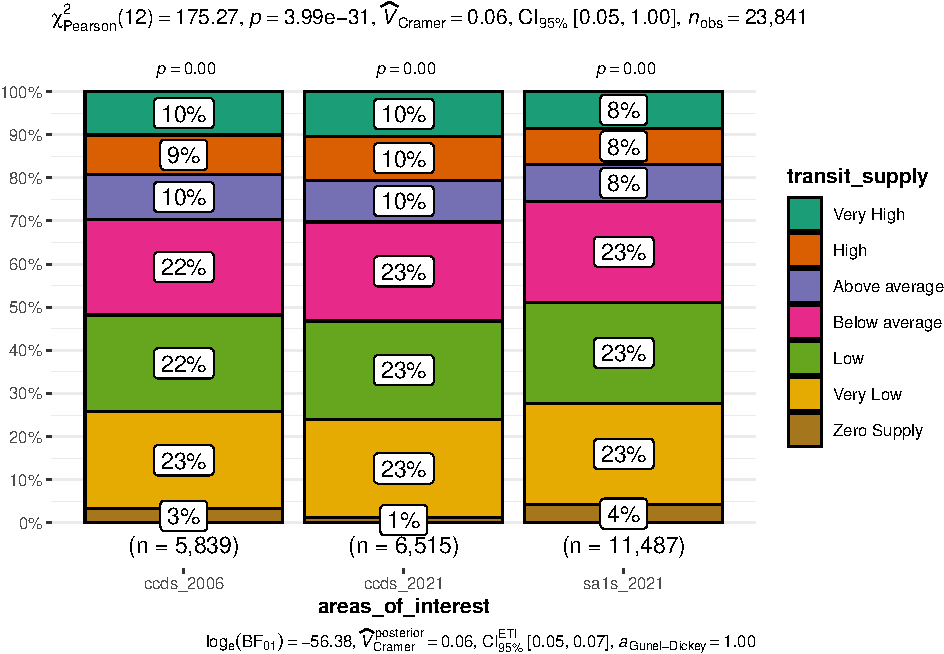
\includegraphics{Leveraging_GTFS_to_assess_transit_supply_Transport_Geography_files/figure-latex/Greater_Melbourne_SA1_2021_table-1.pdf}
\caption{Greater Melbourne: distribution of Transit Supply, 2006 CCDs,
2021 CCDs and 2021 SA1s, population 2006 and 2021. Sources: 2006 values
- Currie (2010), 2021 values - authors}
\end{figure}

Figure \ref{fig:Greater_Melbourne_SA1_2021_plot} shows that there are
still many areas with very low or zero transit supply, especially in
outer areas. Within the 2006 Greater Melbourne boundary there are only
81 CCDs with Zero Supply in 2021, compared to the 186 reported in
\citet{currie2010identifying} for 2006. When including the new parts of
Greater Melbourne, however, there are 489 SA1s with Zero Supply in 2021,
making up 4.3\% of the total number of SA1s in Greater Melbourne,
compared to the 3.2\% of CCDs with Zero Supply in 2006 reported in
\citet{currie2010identifying}. Table
\ref{tab:Greater_Melbourne_SA1_2021_table} and Figure
\ref{fig:Greater_Melbourne_SA1_2021_table} also show that more of the
population of Greater Melbourne are within areas with Zero Supply in
2021 (3.8\%) than in 2006 (2.5\%)

The average SI value has also increased to 3,389.5 from the value of
2,886.9 in 2006 reported in \citet{currie2010identifying}, indicating
that the overall transit service supply score has increased by
approximately 31\%. SI scores average 12,275.7, 3,409.1 and 998.6 for
the inner, middle and outer suburbs respectively\footnote{The same
  grouping of LGAs to inner, middle and outer suburb groups as used in
  \citet{currie2010identifying} was used for this analysis, although
  here the City of Stonnington was allocated entirely to the middle
  grouping, whereas \citet{currie2010identifying} allocated part of this
  LGA to the inner group.}, compared to 10,922.7, 2,694.9 and 764.3,
respectively, reported for 2006 in \citet{currie2010identifying}.

\subsubsection{2021 Social needs}\label{social-needs}

Figure \ref{fig:Greater_Melbourne_2021_social_needs} shows the
distribution of categories of social need index scores across Greater
Melbourne for 2021. This figure is analogous to the 2006 value from
\citet{currie2010identifying} shown in Figure \ref{fig:Currie_map_needs}
although, as discussed in the methodology section above, it was not
possible to exactly replicate the \citet{currie2010identifying} approach
due to changes in the way census results are reported.

\begin{figure}
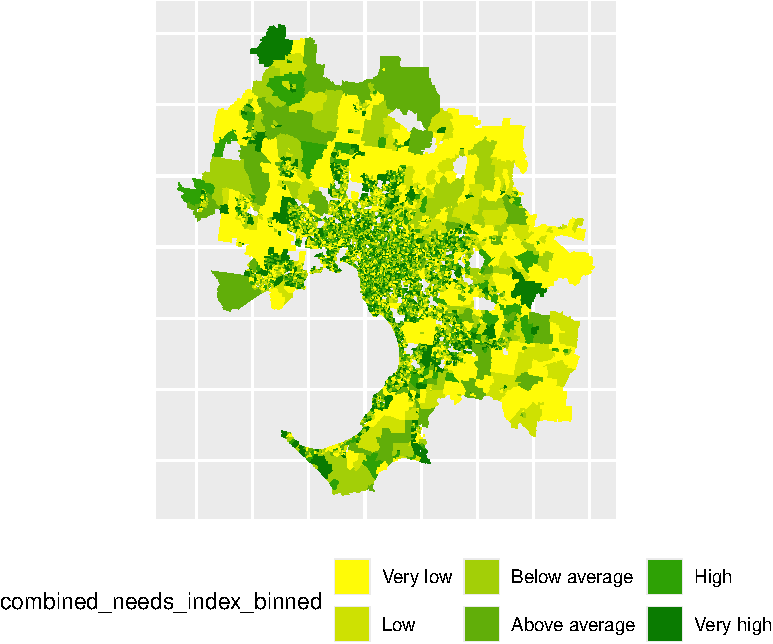
\includegraphics[width=0.9\linewidth]{Leveraging_GTFS_to_assess_transit_supply_Transport_Geography_files/figure-latex/Greater_Melbourne_2021_social_needs-1} \caption{Distribution of categories of composite social need index scores, overlayed with: 2006 Greater Melbourne boundary (black); middle/outer and inner/middle suburb boundaries (grey); and suburban railway lines (dashed).}\label{fig:Greater_Melbourne_2021_social_needs}
\end{figure}

Comparing Figure \ref{fig:Greater_Melbourne_2021_social_needs} and
Figure \ref{fig:Currie_map_needs} suggests that in 2021, compared to
2006: the spatial grouping of different levels of social need is less
consistent; middle eastern suburbs have higher relative needs; and outer
suburbs, particularly in the north-east and south-east, have lower
relative needs. However, this may be an artifact of: the differences in
the composite needs scores used in this analysis (due to the lack of
data to assess relative needs) compared to the
\citet{currie2010identifying} analysis; and the shift of the ABS from
using CCDs to SA1s\footnote{CCDs were originally devised to group the
  approximately 200 dwellings allocated to each individual census
  collector, whereas SA1s were introduced in be consistent in population
  (200 to 800 people, averaging 400) and character\citep{ABS_SA1s_CCDs}}.

\subsubsection{Needs-gap analysis}\label{needs-gap-analysis}

\begin{figure}
\centering
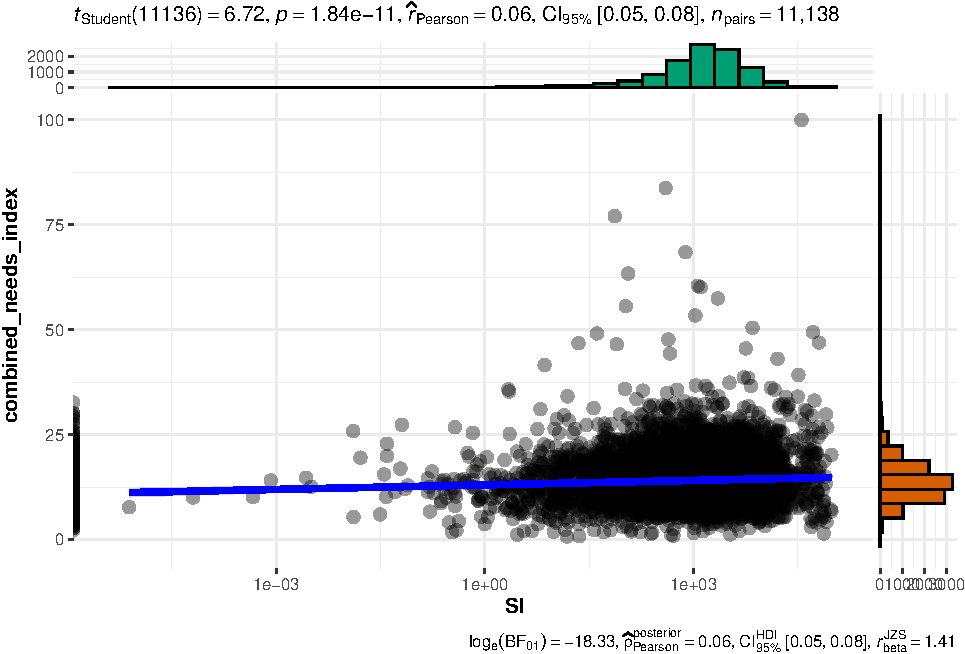
\includegraphics{Leveraging_GTFS_to_assess_transit_supply_Transport_Geography_files/figure-latex/Greater_Melbourne_2021_needs_gap-1.pdf}
\caption{Greater Melbourne 2021, SI and Combined Needs Index scores}
\end{figure}

Figure \ref{fig:Greater_Melbourne_2021_needs_gap} compares SI and
Combined Needs Index scores for SA1s in 2021. There is a significant,
but only weakly positive relationship.

\begin{table}

\caption{\label{tab:Greater_Melbourne_2021_needs_gap_zones}Greater Melbourne 2021, SA1s within each SI and Combined Needs Index grouping}
\centering
\fontsize{8}{10}\selectfont
\begin{tabular}[t]{l|r|r|r|r|r|r|r}
\hline
transit\_supply & Very Low & Low & Below average & Above average & High & Very High & Total\\
\hline
Zero Supply & 6.4\%   (130) & 4.7\%    (95) & 3.9\%    (79) & 2.9\%    (49) & 3.0\%    (51) & 3.6\%    (61) & 4.2\%    (465)\\
\hline
Very Low & 25.6\%   (520) & 22.3\%   (454) & 21.7\%   (442) & 21.0\%   (353) & 22.0\%   (369) & 24.3\%   (408) & 22.9\%  (2,546)\\
\hline
Low & 23.5\%   (478) & 25.3\%   (514) & 24.6\%   (500) & 24.1\%   (404) & 22.4\%   (376) & 20.6\%   (346) & 23.5\%  (2,618)\\
\hline
Below average & 23.7\%   (483) & 23.6\%   (481) & 23.9\%   (487) & 25.6\%   (430) & 24.6\%   (413) & 20.8\%   (350) & 23.7\%  (2,644)\\
\hline
Above average & 6.9\%   (140) & 8.1\%   (165) & 9.2\%   (188) & 9.3\%   (156) & 9.1\%   (152) & 9.2\%   (155) & 8.6\%    (956)\\
\hline
High & 5.9\%   (120) & 7.9\%   (161) & 9.5\%   (194) & 9.2\%   (154) & 9.7\%   (162) & 9.8\%   (165) & 8.6\%    (956)\\
\hline
Very High & 8.0\%   (163) & 8.1\%   (164) & 7.1\%   (144) & 7.9\%   (133) & 9.2\%   (155) & 11.6\%   (194) & 8.6\%    (953)\\
\hline
Total & 100.0\% (2,034) & 100.0\% (2,034) & 100.0\% (2,034) & 100.0\% (1,679) & 100.0\% (1,678) & 100.0\% (1,679) & 100.0\% (11,138)\\
\hline
\end{tabular}
\end{table}

\begin{figure}
\centering
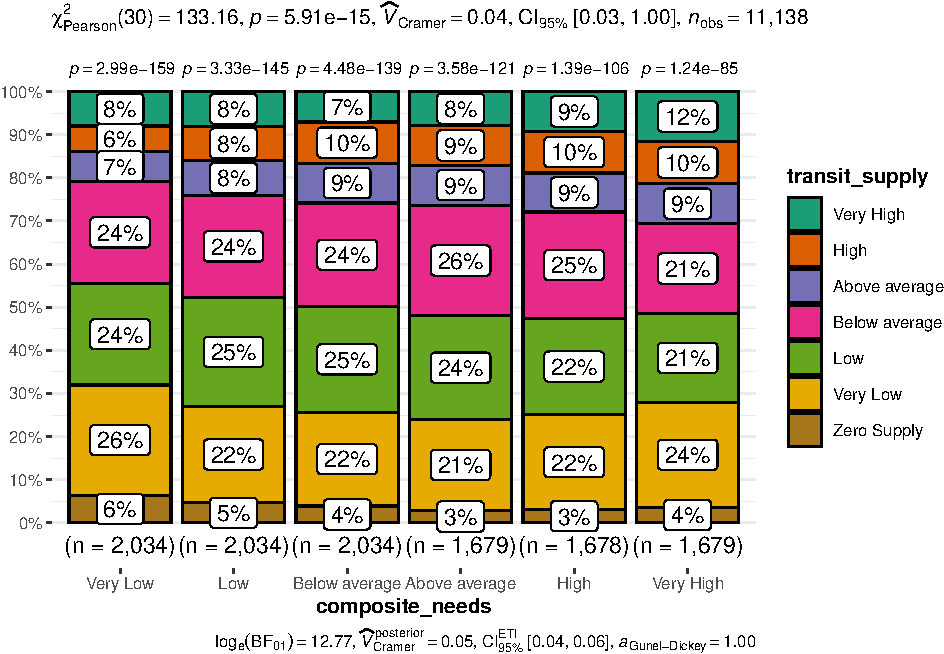
\includegraphics{Leveraging_GTFS_to_assess_transit_supply_Transport_Geography_files/figure-latex/Greater_Melbourne_2021_needs_gap_zones-1.pdf}
\caption{Greater Melbourne 2021, SA1s within each SI and Combined Needs
Index grouping}
\end{figure}

Figure \ref{fig:Greater_Melbourne_2021_needs_gap_zones} and Table
\ref{tab:Greater_Melbourne_2021_needs_gap_zones} compares the SI and
Combined Needs Index groupings for 2021. There is a statistically
significant relationship, although this appears to be weak. 469 SA1s
have zero or very low transit supply, but very high social needs. This
represents 4.2\% of the 11,138 SA1s within Greater Melbourne, and is a
higher proportion than that reported for 2006 (85 of 5,720 CCDs
(1.6\%)).

\begin{table}

\caption{\label{tab:Greater_Melbourne_2021_needs_gap_population}Greater Melbourne 2021, Population in each SI and Combined Needs Index grouping}
\centering
\fontsize{8}{10}\selectfont
\begin{tabular}[t]{l|r|r|r|r|r|r|r}
\hline
transit\_supply & Very Low & Low & Below average & Above average & High & Very High & Total\\
\hline
Zero Supply & 5.7\%  (30,002) & 4.6\%  (32,645) & 3.9\%  (32,328) & 2.9\%  (22,705) & 3.0\%  (27,179) & 3.7\%    (41,915) & 3.8\%   (186,774)\\
\hline
Very Low & 24.4\% (129,294) & 22.4\% (158,919) & 21.7\% (181,719) & 21.1\% (166,490) & 22.3\% (199,467) & 25.6\%   (291,972) & 23.0\% (1,127,861)\\
\hline
Low & 24.6\% (130,477) & 25.8\% (183,274) & 25.1\% (210,538) & 24.5\% (193,642) & 22.9\% (205,397) & 21.0\%   (239,267) & 23.7\% (1,162,595)\\
\hline
Below average & 24.6\% (130,322) & 24.1\% (171,561) & 24.2\% (203,230) & 25.8\% (203,985) & 24.5\% (219,755) & 20.1\%   (229,221) & 23.6\% (1,158,074)\\
\hline
Above average & 7.1\%  (37,419) & 8.0\%  (56,902) & 9.1\%  (76,179) & 9.3\%  (73,062) & 9.0\%  (80,380) & 8.9\%   (100,957) & 8.7\%   (424,899)\\
\hline
High & 6.1\%  (32,274) & 7.6\%  (54,119) & 9.3\%  (77,767) & 8.9\%  (70,132) & 9.4\%  (83,970) & 9.4\%   (107,121) & 8.7\%   (425,383)\\
\hline
Very High & 7.6\%  (40,417) & 7.5\%  (53,477) & 6.7\%  (56,412) & 7.5\%  (59,356) & 8.9\%  (79,306) & 11.4\%   (129,759) & 8.5\%   (418,727)\\
\hline
Total & 100.0\% (530,205) & 100.0\% (710,897) & 100.0\% (838,173) & 100.0\% (789,372) & 100.0\% (895,454) & 100.0\% (1,140,212) & 100.0\% (4,904,313)\\
\hline
\end{tabular}
\end{table}

\begin{figure}
\centering
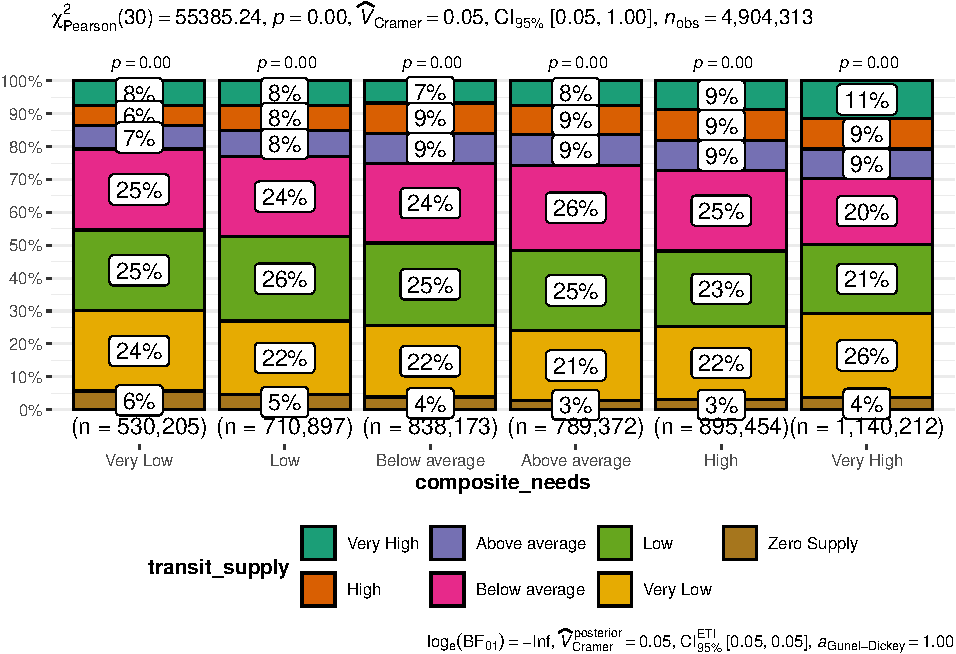
\includegraphics{Leveraging_GTFS_to_assess_transit_supply_Transport_Geography_files/figure-latex/Greater_Melbourne_2021_needs_gap_population-1.pdf}
\caption{Greater Melbourne 2021, Populations within each SI and Combined
Needs Index grouping}
\end{figure}

Figure \ref{fig:Greater_Melbourne_2021_needs_gap_population} and Table
\ref{tab:Greater_Melbourne_2021_needs_gap_population} compares the
populations within each SI and Combined Needs Index grouping for 2021.
There is a statistically significant relationship, although this appears
to be weak. 333887 people live within SA1s that have zero or very low
transit supply, but very high social needs. This represents 6.8\% of the
4,904,313 people within Greater Melbourne, and is a lower proportion
than that reported for 2006 (37,699 of 3.3 million people (8.2\%)).

\begin{figure}
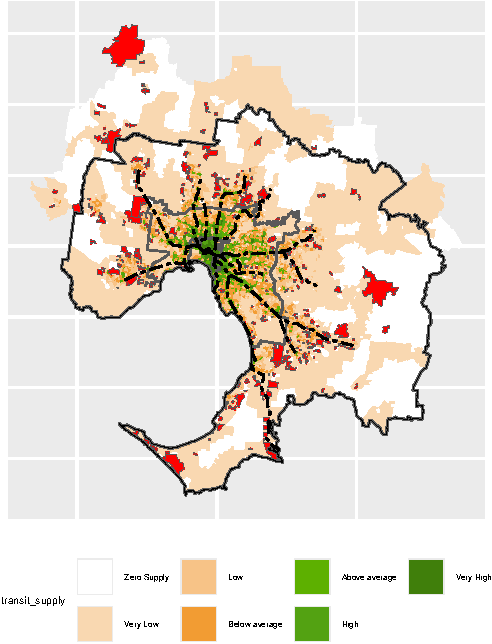
\includegraphics[width=1\linewidth]{Leveraging_GTFS_to_assess_transit_supply_Transport_Geography_files/figure-latex/Greater_Melbourne_2021_needs_gap_map-1} \caption{Greater Melbourne 2021 SI groupings, overlayed with SA1s with very high transport need areas with zero or very low public transport supply (red).}\label{fig:Greater_Melbourne_2021_needs_gap_map}
\end{figure}

Figure \ref{fig:Greater_Melbourne_2021_needs_gap_map} shows SA1 zones in
Greater Melbourne with Very High transport needs, but Very Low or Zero
transit supply. \textless\textless\textless\textless WRITE COMPARISON TO
FIGURE 3
HERE\textgreater\textgreater\textgreater\textgreater\textgreater{}

\subsection{Variation in spatial patterns across Australian
cities}\label{variation-in-spatial-patterns-across-australian-cities}

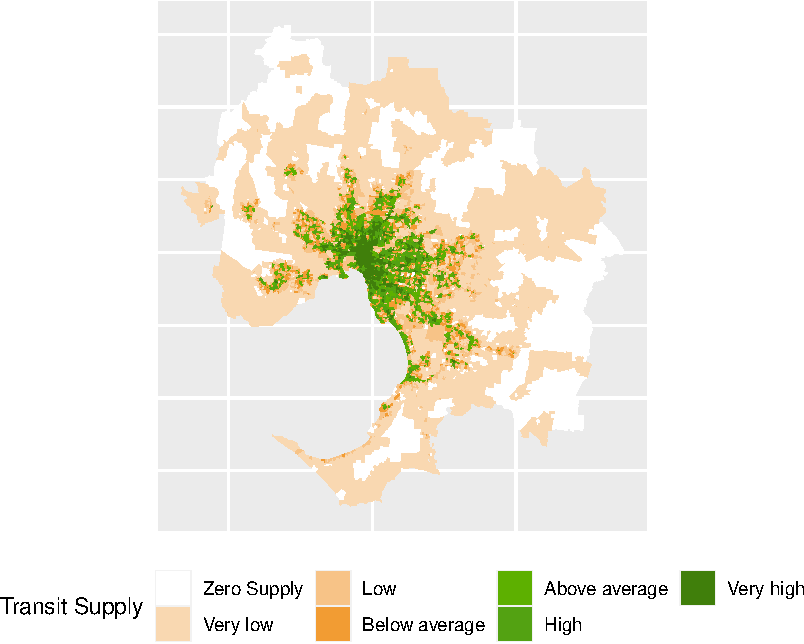
\includegraphics{Leveraging_GTFS_to_assess_transit_supply_Transport_Geography_files/figure-latex/Australian_cities_2021-1.pdf}
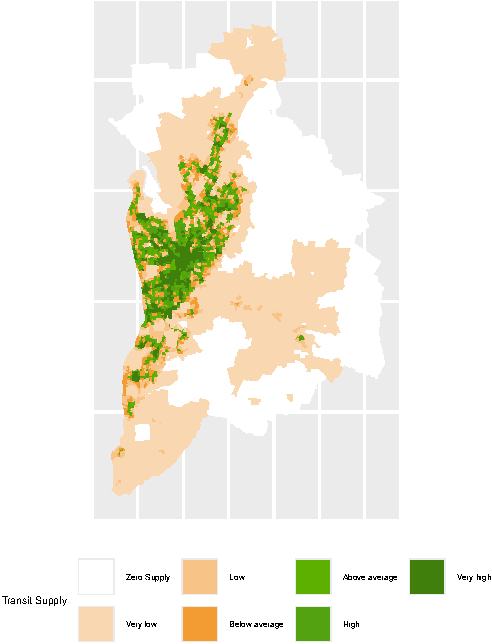
\includegraphics{Leveraging_GTFS_to_assess_transit_supply_Transport_Geography_files/figure-latex/Australian_cities_2021-2.pdf}
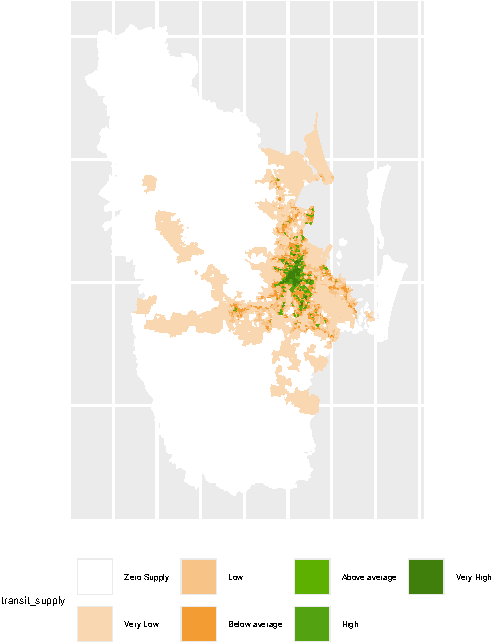
\includegraphics{Leveraging_GTFS_to_assess_transit_supply_Transport_Geography_files/figure-latex/Australian_cities_2021-3.pdf}
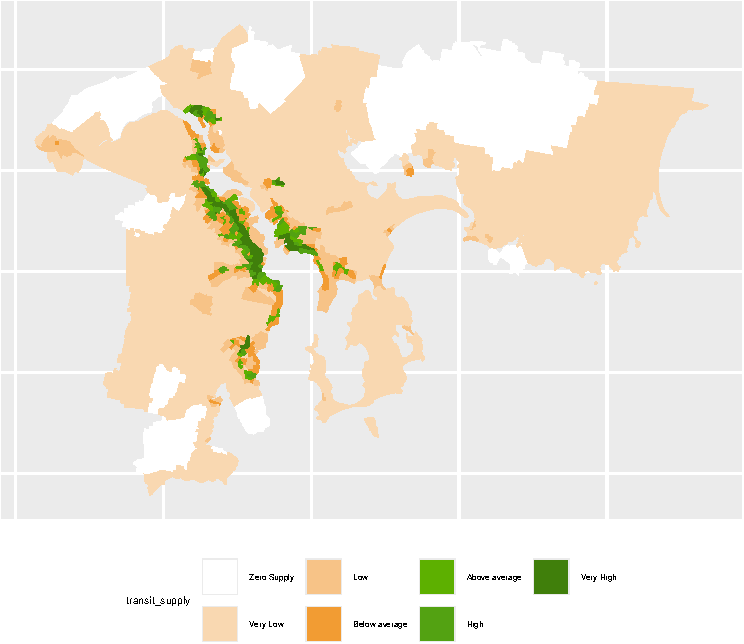
\includegraphics{Leveraging_GTFS_to_assess_transit_supply_Transport_Geography_files/figure-latex/Australian_cities_2021-4.pdf}
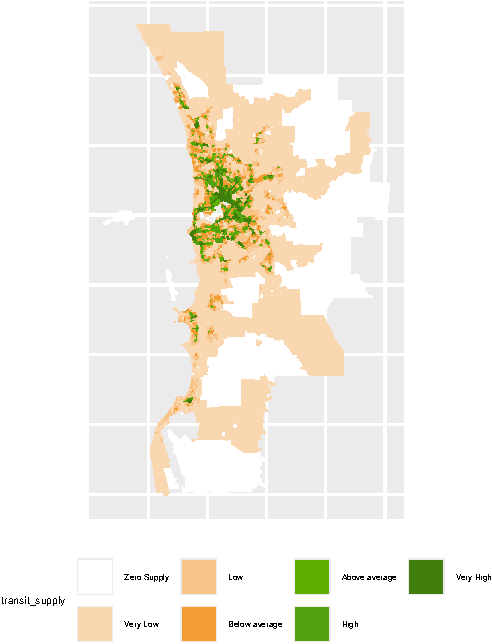
\includegraphics{Leveraging_GTFS_to_assess_transit_supply_Transport_Geography_files/figure-latex/Australian_cities_2021-5.pdf}

Figure \ref{fig:Australian_cities_2021} shows SI values for the week
starting on the day of the 2021 census for all Australian Capital Cities
except Greater Sydney, for which the SI values are calculated for the
week starting .

\section{Discussion}\label{discussion}

\subsection{Limitations}\label{limitations}

\subsection{Directions for furture
research}\label{directions-for-furture-research}

\section{Conclusions}\label{conclusions}

\section*{References}\label{references}
\addcontentsline{toc}{section}{References}

\renewcommand\refname{Appendix A - GCCSA maps by SA1}
\bibliography{References.bib, packages.bib}


\end{document}
